% ++++++++++++ Domain Pi AKS klassen ++++++++++++++
\subsubsection{Domain-klasse: Aks}\label{sec:aks_design}

\begin{figure}[h]
\centering
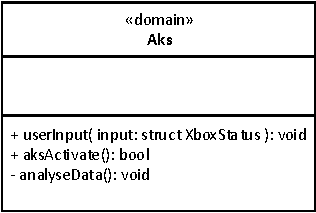
\includegraphics[scale=1]{../fig/diagrammer/bil/cd_aks.pdf}
\caption{Klassebeskrivelse for domain-klassen Aks}
\label{fig:cd_aks}
\end{figure}

\textbf{Attributter}

\begin{table}[h]
\begin{tabularx}{\textwidth}{| Z | Z | L{9cm} |} \hline
Navn & Type & Beskrivelse \\\hline
\texttt{MySteering} & \texttt{Steering} & Styretøjsklassen, bruges når Aks skal påvirke bilens hastighed eller retning.\\\hline
\texttt{MyData} & \texttt{Data*} & Pointer til bilens datastruktur.\\\hline
\texttt{MySettings} & \texttt{Settings*} & Pointer til Settingsklassen. \\\hline
\texttt{MyLog} & \texttt{Log*} & Pointer til loggen. \\\hline
\texttt{state} & \texttt{aksStates} & Husker hvilket stadie bilen er i, kan skifte mellem at stå stille, køre fremad/bagud eller trille. \\\hline
\texttt{proxSensors} & \texttt{int*} & Et array med nuværende værdier fra afstandssensorer \\\hline
\texttt{old\_proxSensors} & \texttt{int*} & Et array der holder de foregående værdier fra afstandssensorer \\\hline
\texttt{latestUserInput} & \texttt{UserInput} & Gemmer de seneste input fra brugeren. \\ \hline
\end{tabularx}
\caption{Attributter for klassen Aks}
\label{table:attr_aks}
\end{table}

\textbf{Metoder}


%----------------- aksActivate -------------------
\begin{table}[h]
\begin{tabularx}{\textwidth}{| L{2.5 cm} | Z |} \hline
Prototype & \texttt{void aksActivate(void)} \\\hline
Parametre & \texttt{void}  \\\hline
Returværdi &  \texttt{bool} \newline Returnerer \texttt{TRUE} hvis det gik godt og \texttt{FALSE} hvis der skete fejl undervejs. \\\hline
Beskrivelse & Metoden kaldes når det automatiske anti-kollisionssystem skal aktiveres. Forhindrer samtidigt input fra brugeren kortvarigt. \\\hline
\end{tabularx}
\caption{Metodebeskrivelse for \texttt{aksActivate}}
\label{table:met_aks_aksActivate}
\end{table}

%----------------- analyseData -------------------
\begin{table}[h]
\begin{tabularx}{\textwidth}{| L{2.5 cm} | Z |} \hline
Prototype & \texttt{void analyseData(void)} \\\hline
Parametre & \texttt{void}  \\\hline
Returværdi &  \texttt{void}  \\\hline
Beskrivelse & Metoden analyserer indhentet data fra Data klassen og vurderer hvilken type af undvigelse der bedst passer. Aktiverer herefter Steering-klassen for at bilen skal undvige forhindringen. \\\hline
\end{tabularx}
\caption{Metodebeskrivelse for \texttt{analyseData}}
\label{table:met_aks_analyseData}
\end{table}